% Experimental design and training protocol (Sec. 3.6), following configs/experiment_0011.yaml.
% Included with \includestandalone (sections/methodology.tex); also compiles alone.
\documentclass[tikz,border=3pt]{standalone}
\usepackage[T1]{fontenc}
\usepackage{newtxtext,newtxmath}
\usetikzlibrary{positioning,arrows.meta,calc,fit,shapes.geometric}

% Same palette as cover_architecture.tex
\definecolor{neural}{HTML}{2F6DB5}
\definecolor{neuralbg}{HTML}{E8F0FA}
\definecolor{symb}{HTML}{D9822B}
\definecolor{symbbg}{HTML}{FCF0E3}
\definecolor{logic}{HTML}{2E8B57}
\definecolor{logicbg}{HTML}{E6F4EC}
\definecolor{relneg}{HTML}{C0392B}

\providecommand{\model}{COVER}
\providecommand{\cls}{\textsc{[cls]}}

\tikzset{
  >={Stealth[length=2mm]},
  flow/.style={->, line width=0.7pt, draw=black!70},
  panel/.style={draw=black!35, rounded corners=4pt, line width=0.6pt},
  title/.style={font=\bfseries\small, anchor=south west, inner sep=1pt},
  card/.style={draw=#1, fill=#1bg, rounded corners=3pt, line width=0.7pt, text width=3.75cm,
               font=\scriptsize, align=left, inner sep=3pt},
  stp/.style={draw=black!55, fill=white, rounded corners=2.5pt, line width=0.6pt, text width=3.6cm,
               font=\scriptsize, align=center, inner sep=2.5pt},
  dec/.style={draw=black!55, fill=black!5, diamond, aspect=2.4, inner sep=0.5pt, font=\scriptsize},
  lab/.style={font=\tiny, fill=white, inner sep=0.8pt},
  setting/.style={draw=black!50, fill=black!4, rounded corners=3pt, line width=0.7pt, text width=3.75cm,
               font=\scriptsize, align=left, inner sep=3pt},
  dot/.style={circle, fill=#1, inner sep=0pt, minimum size=1.9mm},
}

\begin{document}
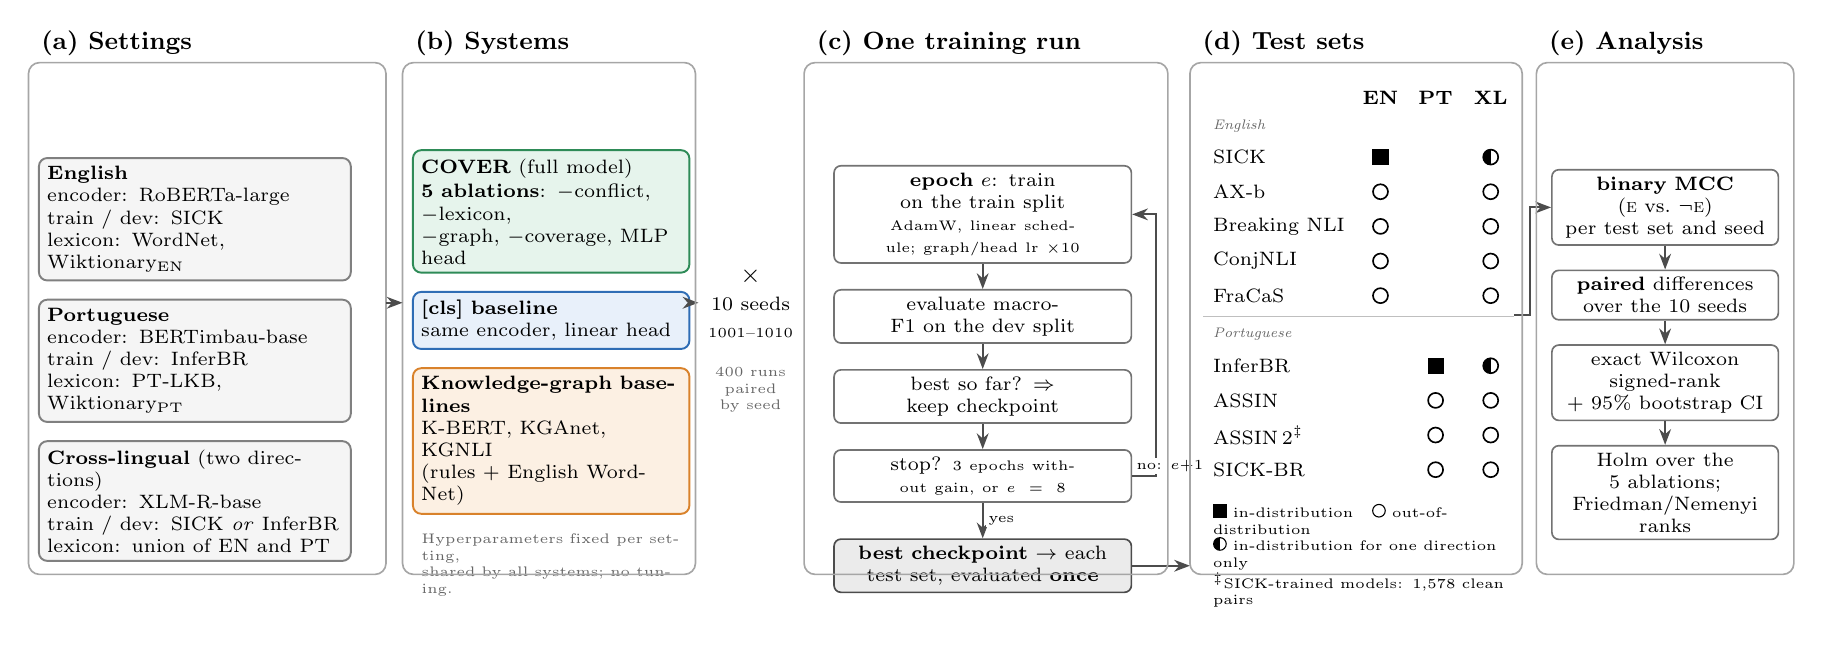
\begin{tikzpicture}

\def\ptop{6.2}
\def\pbot{-0.3}

% =====================================================================
% (a) Settings
% =====================================================================
\node[title] at (0,\ptop+0.05) {(a) Settings};
\node[setting, anchor=north west] (en) at (0,\ptop-1.2) {%
  \textbf{English}\\ encoder: RoBERTa-large\\ train / dev: SICK\\ lexicon: WordNet, Wiktionary\textsubscript{EN}};
\node[setting, anchor=north west] (pt) at ($(en.south west)+(0,-0.22)$) {%
  \textbf{Portuguese}\\ encoder: BERTimbau-base\\ train / dev: InferBR\\ lexicon: PT-LKB, Wiktionary\textsubscript{PT}};
\node[setting, anchor=north west] (xl) at ($(pt.south west)+(0,-0.22)$) {%
  \textbf{Cross-lingual} (two directions)\\ encoder: XLM-R-base\\ train / dev: SICK \emph{or} InferBR\\ lexicon: union of EN and PT};

% =====================================================================
% (b) Systems
% =====================================================================
\def\bx{4.75}
\node[title] at (\bx,\ptop+0.05) {(b) Systems};
\node[card=logic, text width=3.3cm, anchor=north west] (sys1) at (\bx,\ptop-1.1) {%
  \textbf{\model{}} (full model)\\[1pt]
  \textbf{5 ablations}: $-$conflict, $-$lexicon,\\ $-$graph, $-$coverage, MLP head};
\node[card=neural, text width=3.3cm, anchor=north west, ] (sys2) at ($(sys1.south west)+(0,-0.22)$) {%
  \textbf{\cls{} baseline}\\ same encoder, linear head};
\node[card=symb, text width=3.3cm, anchor=north west, ] (sys3) at ($(sys2.south west)+(0,-0.22)$) {%
  \textbf{Knowledge-graph baselines}\\ K-BERT, KGAnet, KGNLI\\ (rules + English WordNet)};
\node[font=\tiny, text=black!60, text width=3.4cm, align=left, anchor=north west]
  at ($(sys3.south west)+(0,-0.12)$) {Hyperparameters fixed per setting,\\ shared by all systems; no tuning.};

% runs counter between (b) and (c)
\node[font=\small, align=center] (runs) at (9.05,3.15) {$\times$\\[-1pt]{\scriptsize 10 seeds}\\[-1pt]{\tiny 1001--1010}};
\draw[flow] (8.35,3.15) -- (runs.west);
\node[font=\tiny, text=black!60, align=center, anchor=north] at (9.05,2.45) {400 runs\\ paired\\ by seed};

% =====================================================================
% (c) One training run
% =====================================================================
\def\cx{9.85}
\node[title] at (\cx,\ptop+0.05) {(c) One training run};
\node[stp, anchor=north west] (s1) at (\cx+0.25,\ptop-1.3)
  {\textbf{epoch} $e$: train on the train split\\ {\tiny AdamW, linear schedule; graph/head lr $\times10$}};
\node[stp, below=0.32cm of s1] (s2) {evaluate macro-F1 on the dev split};
\node[stp, below=0.32cm of s2] (s3) {best so far? $\Rightarrow$ keep checkpoint};
\node[stp, below=0.32cm of s3] (s4) {stop? \tiny 3 epochs without gain, or $e=8$};
\node[stp, fill=black!8, draw=black!70, below=0.45cm of s4] (best) {\textbf{best checkpoint} $\to$ each test set, evaluated \textbf{once}};

\draw[flow] (s1) -- (s2);
\draw[flow] (s2) -- (s3);
\draw[flow] (s3) -- (s4);
\draw[flow] (s4) -- node[lab, right=1pt] {yes} (best);
\draw[flow] (s4.east) -- ++(0.3,0) |- (s1.east);
\node[lab, anchor=south west] at ($(s4.east)+(0.02,0.02)$) {no: $e{+}1$};

% =====================================================================
% (d) Test sets per setting
% =====================================================================
\def\dx{14.75}
\node[title] at (\dx,\ptop+0.05) {(d) Test sets};
\def\cA{17.05}\def\cB{17.75}\def\cC{18.45}
\node[font=\scriptsize\bfseries] at (\cA,5.75) {EN};
\node[font=\scriptsize\bfseries] at (\cB,5.75) {PT};
\node[font=\scriptsize\bfseries] at (\cC,5.75) {XL};
\def\rowstep{0.44}
\newcommand{\trow}[5]{% y, name, EN, PT, XL  (i = in-distribution, o = out-of-distribution, - = not run)
  \node[font=\scriptsize, anchor=west] at (\dx+0.05,#1) {#2};
  \foreach \c/\v in {\cA/#3,\cB/#4,\cC/#5}{%
    \if i\v \node[draw=black, fill=black, inner sep=0pt, minimum size=1.9mm] at (\c,#1) {};\fi
    \if o\v \node[dot=black!0, draw=black, line width=0.6pt] at (\c,#1) {};\fi
    \if h\v \node[circle, draw=black, line width=0.6pt, inner sep=0pt, minimum size=1.9mm,
                  path picture={\fill[black] (path picture bounding box.south west) rectangle
                  (path picture bounding box.north);}] at (\c,#1) {};\fi
  }%
}
\node[font=\tiny\itshape, text=black!60, anchor=west] at (\dx+0.05,5.4) {English};
\trow{5.0}{SICK}{i}{-}{h}
\trow{4.56}{AX-b}{o}{-}{o}
\trow{4.12}{Breaking NLI}{o}{-}{o}
\trow{3.68}{ConjNLI}{o}{-}{o}
\trow{3.24}{FraCaS}{o}{-}{o}
\draw[black!25] (\dx+0.05,2.98) -- (18.75,2.98);
\node[font=\tiny\itshape, text=black!60, anchor=west] at (\dx+0.05,2.75) {Portuguese};
\trow{2.35}{InferBR}{-}{i}{h}
\trow{1.91}{ASSIN}{-}{o}{o}
\trow{1.47}{ASSIN\,2$^{\ddagger}$}{-}{o}{o}
\trow{1.03}{SICK-BR}{-}{o}{o}
\node[font=\tiny, align=left, anchor=north west, text width=4cm] at (\dx+0.05,0.72) {%
  \tikz\node[draw=black, fill=black, inner sep=0pt, minimum size=1.6mm]{}; in-distribution\quad
  \tikz\node[circle, draw=black, inner sep=0pt, minimum size=1.6mm]{}; out-of-distribution\\
  \tikz\node[circle, draw=black, inner sep=0pt, minimum size=1.6mm, path picture={\fill[black]
  (path picture bounding box.south west) rectangle (path picture bounding box.north);}]{};
  in-distribution for one direction only\\
  $^{\ddagger}$SICK-trained models: 1{,}578 clean pairs};

\draw[flow] (best.east) -- (best.east -| 14.63,0);

% =====================================================================
% (e) Analysis
% =====================================================================
\def\ex{19.15}
\node[title] at (\ex,\ptop+0.05) {(e) Analysis};
\node[stp, text width=2.7cm, anchor=north] (e1) at ({(19.03+22.3)/2},\ptop-1.35)
  {\textbf{binary MCC} (\textsc{e} vs.\ $\neg$\textsc{e})\\ per test set and seed};
\node[stp, text width=2.7cm, below=0.3cm of e1] (e2)
  {\textbf{paired} differences over the 10 seeds};
\node[stp, text width=2.7cm, below=0.3cm of e2] (e3)
  {exact Wilcoxon signed-rank\\ + 95\% bootstrap CI};
\node[stp, text width=2.7cm, below=0.3cm of e3] (e4)
  {Holm over the 5 ablations;\\ Friedman/Nemenyi ranks};
\draw[flow] (e1) -- (e2);
\draw[flow] (e2) -- (e3);
\draw[flow] (e3) -- (e4);
\draw[flow] (18.75,3.0) -- ++(0.2,0) |- (e1.west);

% =====================================================================
% panel frames
% =====================================================================
\draw[panel] (-0.12,\pbot) rectangle (4.42,\ptop);
\draw[panel] (4.63,\pbot) rectangle (8.35,\ptop);
\draw[panel] (9.73,\pbot) rectangle (14.35,\ptop);
\draw[panel] (14.63,\pbot) rectangle (18.85,\ptop);
\draw[panel] (19.03,\pbot) rectangle (22.3,\ptop);
\draw[flow] (4.42,3.15) -- (4.63,3.15);

\end{tikzpicture}
\end{document}
